\documentclass{beamer}
%% \documentclass[draft]{beamer} %% draft version

%% restrict generation of slides
%% \includeonlyframes{oligoarray,probesyn}

\mode<presentation>
{
  \usetheme{Bielefeld}
  \setbeamercovered{transparent}
}

\usepackage[english]{babel}
\usepackage[latin1]{inputenc}
\usepackage{graphicx}

\usepackage{lmodern}
\usepackage[T1]{fontenc}

\newcommand{\ignore}[1]{}

\title[Improving Microarray Layout: Pivot Partitioning] % (optional, use only with long paper titles)
{Improving the Layout of Oligonucleotide Microarrays: Pivot Partitioning}

%% \subtitle
%% {Include Only If Paper Has a Subtitle}

\author[S.~A.~de~Carvalho~Jr. (Universit\"at Bielefeld)] % (optional, use only with lots of authors)
{S\'ergio A. de Carvalho Jr.\inst{1,}\inst{2}\inst{,3} \and Sven Rahmann\inst{1,}\inst{2}}
% - Give the names in the same order as the appear in the paper.
% - Use the \inst{?} command only if the authors have different
%   affiliation.

\institute[Universit\"{a}t Bielefeld] % (optional, but mostly needed)
{
\inst{1}%
Algorithms and Statistics for Systems Biology, Genome Informatics,\\
Technische Fakult\"at, Universit\"at Bielefeld, Germany
\and
\inst{2}%
International NRW Graduate School in Bioinformatics and Genome Research
\and
\inst{3}%
Graduiertenkolleg Bioinformatik
}
% - Use the \inst command only if there are several affiliations.
% - Keep it simple, no one is interested in your street address.

\date[WABI 2006] % (optional, should be abbreviation of conference name)
{6th Workshop on Algorithms in Bioinformatics\\Z\"urich, Sep 2006}
% - Either use conference name or its abbreviation.
% - Not really informative to the audience, more for people (including
%   yourself) who are reading the slides online

% \subject{Theoretical Computer Science}
% This is only inserted into the PDF information catalog. Can be left
% out. 

% If you have a file called "university-logo-filename.xxx", where xxx
% is a graphic format that can be processed by latex or pdflatex,
% resp., then you can add a logo as follows:

% \pgfdeclareimage[height=0.5cm]{university-logo}{university-logo-filename}
% \logo{\pgfuseimage{university-logo}}

% Delete this, if you do not want the table of contents to pop up at
% the beginning of each subsection:
\AtBeginSubsection[]
{
  \begin{frame}<beamer>
    \frametitle{Outline}
    \tableofcontents[currentsection,hideallsubsections]
  \end{frame}
}

% If you wish to uncover everything in a step-wise fashion, uncomment
% the following command: 
%\beamerdefaultoverlayspecification{<+->}


\begin{document}

%%%%%%%%%%%%%%%%%%%%%%%%%%%%%%%%%%%%%%%%%%%%%%%%%%%%%%%%%%%%%%%%%%%%%%%%%%%%%%%%
\frame[plain]{

  \vspace*{0.4cm}
  \centerline{
    
\includegraphics[height=1.5cm]{aggi_logo.png}
    \hspace*{2cm}
    
\includegraphics[height=1.5cm]{aggi_logo.png}
  }
  
  \titlepage
}

%%%%%%%%%%%%%%%%%%%%%%%%%%%%%%%%%%%%%%%%%%%%%%%%%%%%%%%%%%%%%%%%%%%%%%%%%%%%%%%%
\frame{\frametitle{Outline}

  \tableofcontents[hideallsubsections]

}

%% *****************************************************************************
\section[Introduction]{Introduction: Microarray Layout}
\subsection{Dummy}
%% *****************************************************************************

%%%%%%%%%%%%%%%%%%%%%%%%%%%%%%%%%%%%%%%%%%%%%%%%%%%%%%%%%%%%%%%%%%%%%%%%%%%%%%%%
\frame[label=oligoarray]{\frametitle{High-Density Oligonucleotide Microarrays}

  \centerline{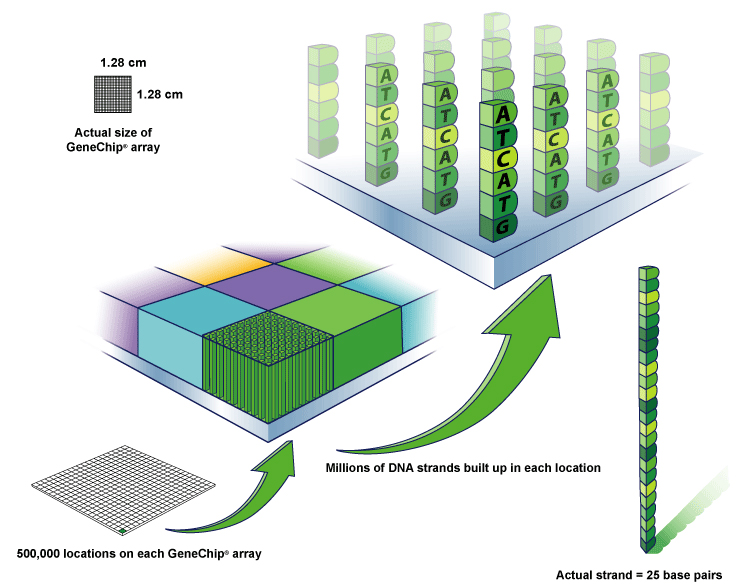
\includegraphics[height=0.9\textheight]{oligoarray.jpg}}
  \vspace*{-0.5cm}
  \centerline{\tiny{Source: Affymetrix, Inc.}}

}

%%%%%%%%%%%%%%%%%%%%%%%%%%%%%%%%%%%%%%%%%%%%%%%%%%%%%%%%%%%%%%%%%%%%%%%%%%%%%%%%
\frame[label=probesyn]{\frametitle{Probe Synthesis: Photolitographic Masks}

  \vspace*{-0.5cm}
  \flushright{\tiny{Source: Affymetrix, Inc.}}
  \centerline{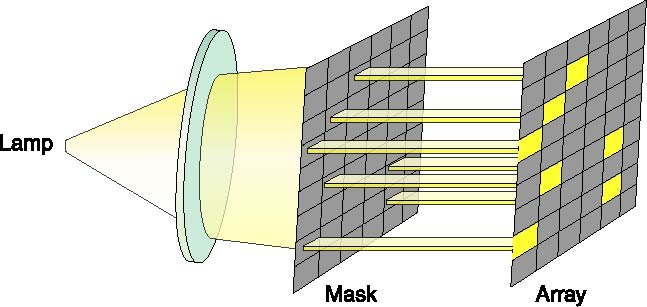
\includegraphics[height=0.5\textheight]{photolitography.jpg}}  

  \begin{itemize}
    \item Probes are synthesized on the chip in a series of \alert{steps}
    \item Each step appends a particular nucleotide to \alert{selected regions}
    \item Selection occurs by exposure to light
  \end{itemize}
}

%%%%%%%%%%%%%%%%%%%%%%%%%%%%%%%%%%%%%%%%%%%%%%%%%%%%%%%%%%%%%%%%%%%%%%%%%%%%%%%%
\frame[label=embed]{\frametitle{Deposition Sequence and Probe Embeddings}

  Show animation with masks

}


%%%%%%%%%%%%%%%%%%%%%%%%%%%%%%%%%%%%%%%%%%%%%%%%%%%%%%%%%%%%%%%%%%%%%%%%%%%%%%%%
\frame[label=problem]{\frametitle{Problem: Unintended Illumination}

  \begin{block}{Border Length Minimization Problem}
  \end{block}

}

%% *****************************************************************************
\section[Conflict Index]{Conflict Index Evaluation Model}
\subsection{Dummy}
%% *****************************************************************************

%%%%%%%%%%%%%%%%%%%%%%%%%%%%%%%%%%%%%%%%%%%%%%%%%%%%%%%%%%%%%%%%%%%%%%%%%%%%%%%%
\frame{\frametitle{Motivation}
}

%% *****************************************************************************
\section[Pivot Partitioning]{Pivot Partitioning Algorithm}
\subsection{Dummy}
%% *****************************************************************************

%%%%%%%%%%%%%%%%%%%%%%%%%%%%%%%%%%%%%%%%%%%%%%%%%%%%%%%%%%%%%%%%%%%%%%%%%%%%%%%%
\frame{\frametitle{Previous work}
}

%% *****************************************************************************
\section*{Summary}
\subsection*{Dummy}
%% *****************************************************************************

%%%%%%%%%%%%%%%%%%%%%%%%%%%%%%%%%%%%%%%%%%%%%%%%%%%%%%%%%%%%%%%%%%%%%%%%%%%%%%%%
\frame{\frametitle{Summary}
}

%%%%%%%%%%%%%%%%%%%%%%%%%%%%%%%%%%%%%%%%%%%%%%%%%%%%%%%%%%%%%%%%%%%%%%%%%%%%%%%%
\begin{frame}{Thanks!}

  \centerline{
    
\includegraphics[height=1.5cm]{aggi_logo.png}
    \hspace*{2cm}
    
\includegraphics[height=1.5cm]{aggi_logo.png}
  }

  \vspace*{0.5cm}
  \begin{itemize}
    \item Prof. Dr. Jens Stoye
    \item Prof. Dr. Robert Giegerich
    \item AG Genominformatik
    \item Graduiertenkolleg Bioinformatik
    \item Graduate School in Bioinformatics and Genome Research
  \end{itemize}
  
  \vskip0pt plus.5fill
  \centerline{\alert{Thank you for your attention!}}
  
\end{frame}

\end{document}
